\documentclass{article}
\usepackage{amsmath}
\usepackage{graphicx}
\usepackage{array}
\usepackage{amssymb}
\usepackage[margin=1.2in]{geometry}

\begin{document}


\section{Adversarial nets}
The adversarial modeling framework is most straightforward to apply when the models are both multilayer perceptrons.
To learn the generator’s distribution pg over data x, we define a prior on input noise variables $p_z (z)$, 
then represent a mapping to data space as $G(z; \theta g )$, where G is a
differentiable function represented by a multilayer perceptron with parameters $\theta_g$ . We also define a
second multilayer perceptron $D(x; \theta d)$ that outputs a single scalar. $D(x)$ represents the probability
that x came from the data rather than pg . We train D to maximize the probability of assigning the
correct label to both training examples and samples from G. We simultaneously train G to minimize
$\log(1 - D(G(z)))$:


In other words, D and G play the following two-player minimax game with value function V (G, D):

\[
    \min_{G} \max_{D} V(D, G) = \mathbb{E}_{x\sim p_{data}}[\log D(x))] 
    + \mathbb{E}_{z\sim p_z(z)}[\log(1-D(G(z)))]
    \label{eqn1}
\]

\setlength{\parskip}{1em}
\noindent
In the next section, we present a theoretical analysis of adversarial nets, essentially showing that
the training criterion allows one to recover the data generating distribution as G and D are given
enough capacity, i.e., in the non-parametric limit. See Figure 1 for a less formal, more pedagogical
explanation of the approach. In practice, we must implement the game using an iterative, numerical
approach. Optimizing D to completion in the inner loop of training is computationally prohibitive,
and on finite datasets would result in overfitting. Instead, we alternate between k steps of optimizing
D and one step of optimizing G. This results in D being maintained near its optimal solution, so
long as G changes slowly enough. This strategy is analogous to the way that SML/PCD [31, 29]
training maintains samples from a Markov chain from one learning step to the next in order to avoid
burning in a Markov chain as part of the inner loop of learning. The procedure is formally presented
in Algorithm 1.

\setlength{\parskip}{1em}
\noindent
In practice, equation 1 may not provide sufficient gradient for G to learn well. Early in learning,
when G is poor, D can reject samples with high confidence because they are clearly different from
the training data. In this case, $\log(1 - D(G(z)))$ saturates. Rather than training G to minimize
$\log(1 - D(G(z)))$ we can train G to maximize log $D(G(z))$. This objective function results in the
same fixed point of the dynamics of G and D but provides much stronger gradients early in learning.

\begin{figure}[h]
    \centering
    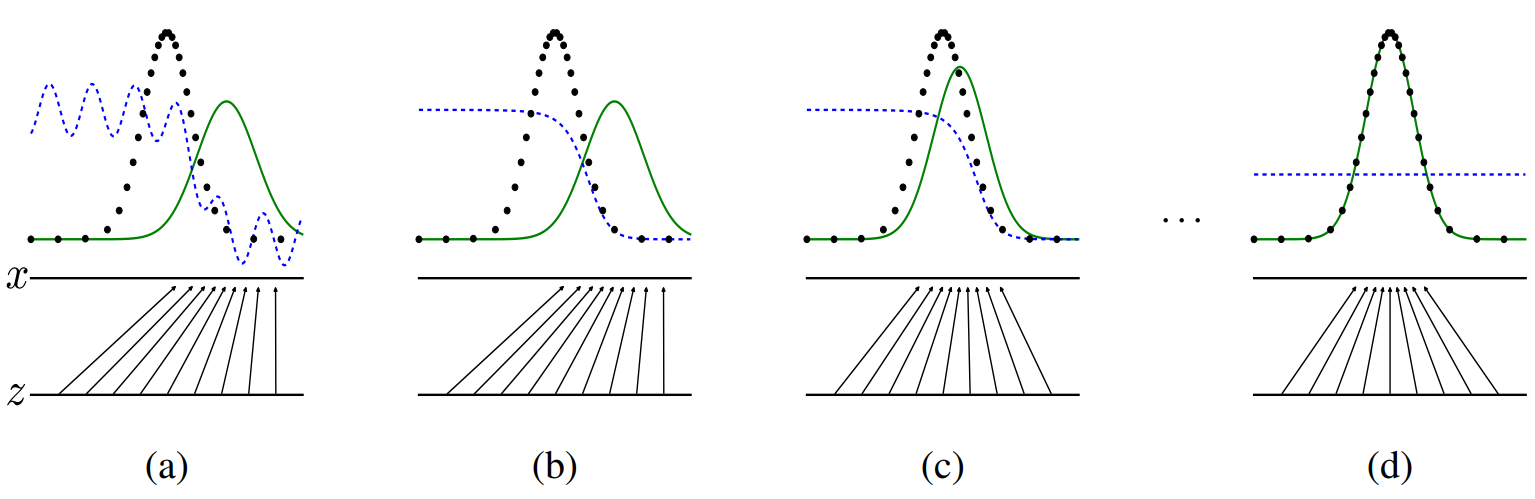
\includegraphics[width=\textwidth]{figure/fig1.PNG}
    \label{fig:fig1}
    \caption{Generative adversarial nets are trained by simultaneously updating the discriminative distribution
(D, blue, dashed line) so that it discriminates between samples from the data generating distribution (black,
dotted line) px from those of the generative distribution pg (G) (green, solid line). The lower horizontal line is
the domain from which z is sampled, in this case uniformly. The horizontal line above is part of the domain
of x. The upward arrows show how the mapping $x = G(z)$ imposes the non-uniform distribution pg on
transformed samples. G contracts in regions of high density and expands in regions of low density of pg. (a)
Consider an adversarial pair near convergence: $p_g$ is similar to pdata and D is a partially accurate classifier.
(b) In the inner loop of the algorithm D is trained to discriminate samples from data, converging to $D^*(x)= \frac{P_{data}(x)}{P_{data}(x)+P_{g}(x)}$  (c) After an update to G, gradient of D has guided G(z) to flow to regions that are more likely
to be classified as data. (d) After several steps of training, if G and D have enough capacity, they will reach a
point at which both cannot improve because $p_g = p_{data}$. The discriminator is unable to differentiate between
the two distributions, i.e. $D(x) = \frac{1}{2}$
}
\end{figure}

\section{Theoretical Results}

The generator G implicitly defines a probability distribution pg as the distribution of the samples
$G(z)$ obtained when $z \sim p_z$. Therefore, we would like Algorithm 1 to converge to a good estimator
of pdata, if given enough capacity and training time. The results of this section are done in a nonparametric
setting, e.g. we represent a model with infinite capacity by studying convergence in the
space of probability density functions.

\setlength{\parskip}{1em}
\noindent
We will show in section 4.1 that this minimax game has a global optimum for pg = pdata. We will
then show in section 4.2 that Algorithm 1 optimizes Eq 1, thus obtaining the desired result.

\begin{table}[h]
    \begin{tabular*}{\textwidth}{p{\textwidth}} \\ \hline
        \textbf{Algorithm} 1 Minibatch stochastic gradient descent training of generative adversarial nets. The number of
       steps to apply to the discriminator, k, is a hyperparameter. We used $k = 1$, the least expensive option, in our
       experiments. 
       \\ \hline
   \end{tabular*}
\end{table}


\subsection{ Global Optimality of $p_g = p_{data}$}    
We first consider the optimal discriminator D for any given generator G.\\
\textbf{Proposition 1}. \textit{For G fixed, the optimal discriminator D is}

\[
D^*(x)= \frac{P_{data}(x)}{P_{data}(x)+P_{g}(x)}
\]

\textit{Proof}. The training criterion for the discriminator D, given any generator G, is to maximize the quantity $V (G, D)$

\begin{equation}
    \begin{split}
      V(G, D) & =    \int_{x}^{}  p_{data}(x)log(D(x))\,dx + \int_{z}^{}  p_{z}(z)log(1-D(g(z)))\,dz \\
      & = \int_{x}^{}  p_{data}(x)log(D(x)) + p_{g}(x)log(1-D(g(x)))\,dx
    \end{split}
\end{equation}

For any $(a, b) \in \mathbb{R}^2 \ \{0, 0\}$, the function 
$y \rightarrow  a log(y) + b log(1 - y)$ 
achieves its maximum in
[0, 1] at $\frac{a}{a+b}$. The discriminator does not need to be defined outside of 
$Supp(p_{data}) \cup Supp(p_g)$,
concluding the proof.
    
\section{Experiments}
We trained adversarial nets an a range of datasets including MNIST[23], the Toronto Face Database
(TFD) [28], and CIFAR-10 [21]. The generator nets used a mixture of rectifier linear activations [19,
9] and sigmoid activations, while the discriminator net used maxout [10] activations. Dropout [17]
was applied in training the discriminator net. While our theoretical framework permits the use of
dropout and other noise at intermediate layers of the generator, we used noise as the input to only
the bottommost layer of the generator network.

\setlength{\parskip}{1em}
\noindent
We estimate probability of the test set data under pg by fitting a Gaussian Parzen 
window to then samples generated with G and reporting the log-likelihood under 
this distribution. The $\sigma$ parameter

\begin{table}[h]
    \centering
    \begin{tabular}{c|c|c} \\
        Model & MNIST & TFD \\ \hline
        DBN [3] & 138 ± 2 & 1909 ± 66 \\  
        Stacked CAE [3] & 121 ± 1.6 & 2110 ± 50 \\
        Deep GSN [6] & 214 ± 1.1 & 1890 ± 29 \\
        Adversarial nets & 225 ± 2 & 2057 ± 26
    \end{tabular}
    \caption{Parzen window-based log-likelihood estimates. The reported numbers on MNIST are 
    the mean loglikelihood of samples on test set, with the standard error of the mean computed 
    across examples. On TFD, we computed the standard error across folds of the dataset,
    with a different $\sigma$ chosen using the validation set of each fold. On TFD, $\sigma$ was
    cross validated on each fold and mean log-likelihood on each fold were computed. For MNIST 
    we compare against other models of the real-valued (rather than binary) 
    version of dataset.}
    \label{tab:my_label}
\end{table}

of the Gaussians was obtained by cross validation on the validation set. This procedure was introduced in Breuleux et al. [8] and used for various generative models for which the exact likelihood
is not tractable [25, 3, 5]. Results are reported in Table 1. This method of estimating the likelihood
has somewhat high variance and does not perform well in high dimensional spaces but it is the best
method available to our knowledge. Advances in generative models that can sample but not estimate
likelihood directly motivate further research into how to evaluate such models.

\setlength{\parskip}{1em}
\noindent
In Figures 2 and 3 we show samples drawn from the generator net after training. While we make no
claim that these samples are better than samples generated by existing methods, we believe that these
samples are at least competitive with the better generative models in the literature and highlight the
potential of the adversarial framework.

\begin{figure}[h]
    \centering
    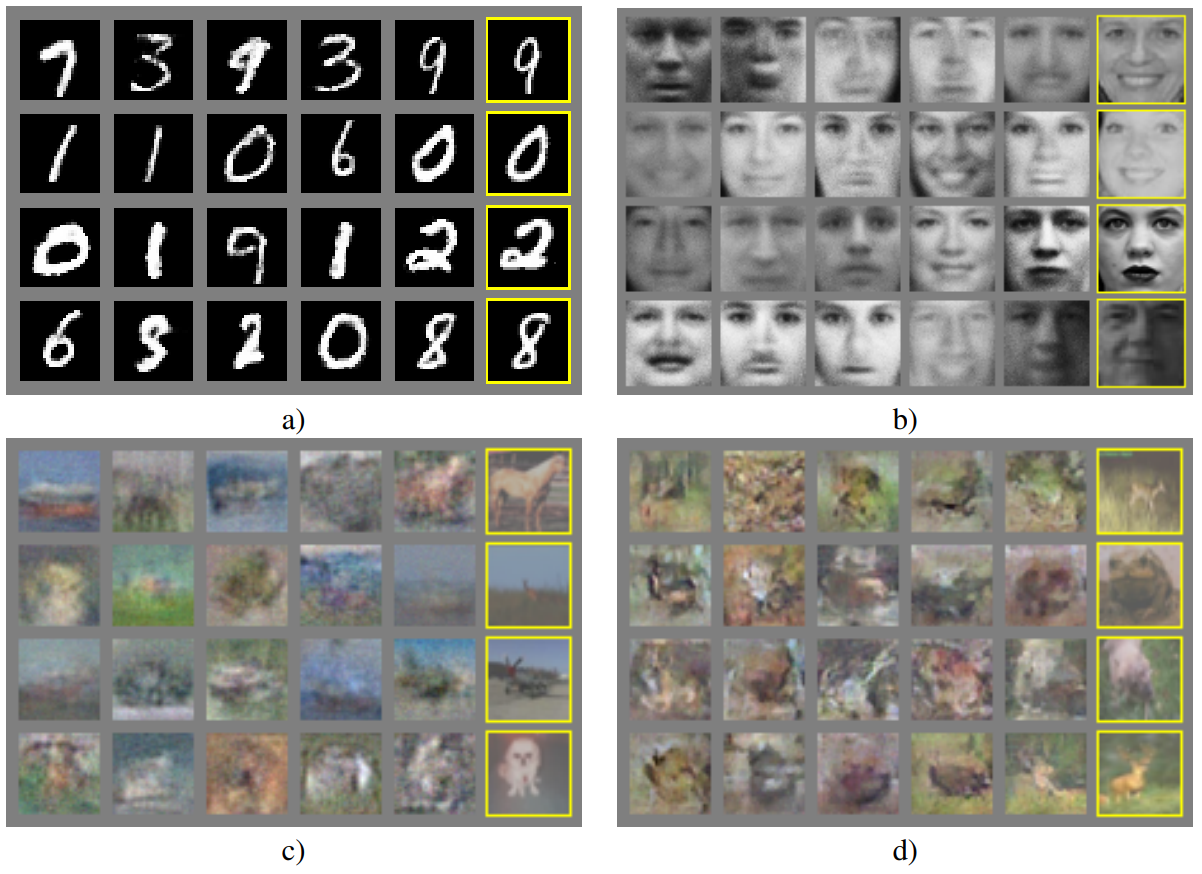
\includegraphics[width=\textwidth]{figure/fig2.PNG}
    \label{fig:fig2}
    \caption{Visualization of samples from the model. Rightmost column shows the nearest training example of
the neighboring sample, in order to demonstrate that the model has not memorized the training set. Samples
are fair random draws, not cherry-picked. Unlike most other visualizations of deep generative models, these
images show actual samples from the model distributions, not conditional means given samples of hidden units.
Moreover, these samples are uncorrelated because the sampling process does not depend on Markov chain
mixing. a) MNIST b) TFD c) CIFAR-10 (fully connected model) d) CIFAR-10 (convolutional discriminator
and “deconvolutional” generator)}
\end{figure}

\begin{figure}[h]
    \centering
    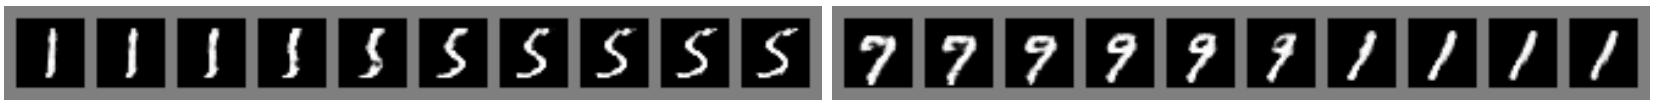
\includegraphics[width=\textwidth]{figure/fig3.PNG}
    \label{fig:fig3}
    \caption{Digits obtained by linearly interpolating between coordinates in z space of the full model.}
\end{figure}
\newpage
\begin{table}[h]
    \begin{tabular*}{\textwidth}{c|p{3cm}|p{3cm}|p{3cm}|l} \\
        & Deep directed graphical models &
        Deep undirected graphical models &
        Generative autoencoders & Adversarial models\\ \hline
        DBN [3] & 138 ± 2 & 1909 ± 66 \\  
        Stacked CAE [3] & 121 ± 1.6 & 2110 ± 50 \\
        Deep GSN [6] & 214 ± 1.1 & 1890 ± 29 \\
        Adversarial nets & 225 ± 2 & 2057 ± 26
    \end{tabular*}
    \caption{Challenges in generative modeling: a summary of the difficulties encountered by different approaches
to deep generative modeling for each of the major operations involving a model.}
    \label{tab:my_label2}
\end{table}


\end{document}
